\section{Multilayer perceptron}


Dans ce  exercice, nous devons impl�menter un reseaux des neurones. Pour faire cela on doit indiquer inidquer le nombre d'entr�e des notres features, le nombre des neurones presents dans la couche cach� et le nombre de  sortie.

Ensuite il a fallu mettre en place le backpropagatoin trainer \texttt{BackProrpTraing} qui s'occupe d'entrener notre reseaux de neurones avec le dataset de trainining et deux paramentres: \texttt{momentum} et le \texttt{learning rate}. 

Pour commencer l'entrainement du reseaux de neuron on appelle ensuite \texttt{trainer.train()} qui execute un \texttt{epoche} d'entrainement u reseaux de neurones.

Voici donc le code de cette exercices :
\lstinputlisting{code/FNN.py}
\newpage


Avec l'entrainement par default on a en resultat un \texttt{precision de 0.55} un \texttt{recall de 0.67} et un  \texttt{f-score de 0.60}.
La matrice de confision \cite{mat001} nous montre aussi que le classe sont pas bienne reconnu par le classificateur:
\begin{figure}[h]
  \centering
    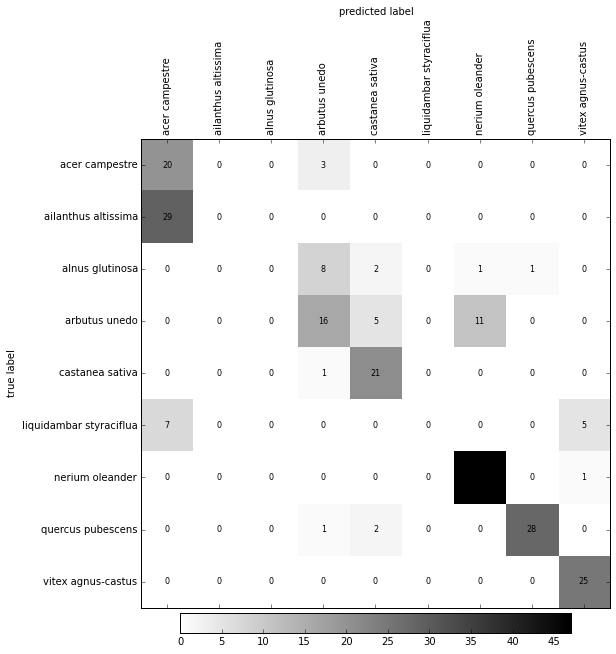
\includegraphics[width=0.6\linewidth]{img/mconf_001.png}
  \caption{Matrice de confusione avec learning rate 0.001 et 50 iterations}
  \label{mat001}
\end{figure}
\newpage


On a du donc tuner cetes paramentres pour ammeliorer les resultats.

on a commencer a modifier le training rate a \texttt{trainintrate=0.1} pour chercher d'ammeliorer plus rapidement l'errerr gen�er� par le'ntrainment et arriver a de meilleures results. 


Par contre, comme on pou voire du graphique  \cite{graph1} l'erreur d'entrainement est assasi instable, cela n'est pas preferable pour trouver un bonne convergence. 
\begin{figure}[h]
  \centering
    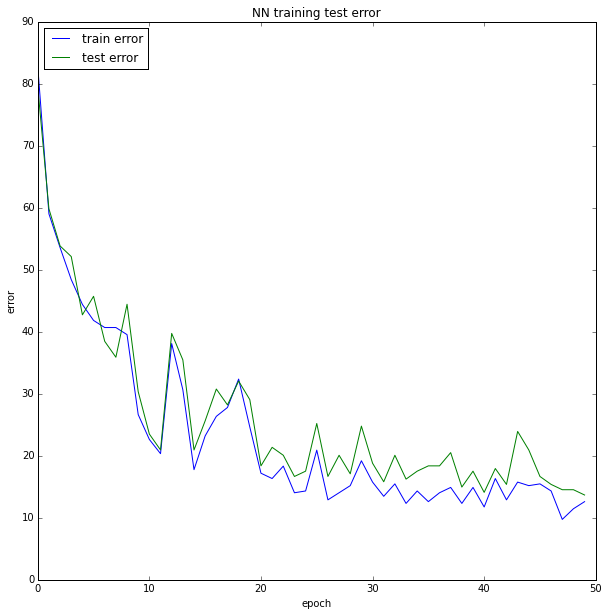
\includegraphics[width=0.6\linewidth]{img/graph1.png}
  \caption{Erreur d'entrainement et de test}
  \label{graph1}
\end{figure}



Nous avons donc essey� plusieurs paralemtnre et en final on a trouv� certen qui parait le meilleurs. 
En final on a execut� \texttt{150 iterations} avec un \texttt{momentum=0.1} et le \texttt{learningrate=0.03}.

On a eu en resultat un \texttt{precision de 0.82} un \texttt{recall de 0.86} et un  \texttt{f-score de 0.84}.

Le graphiqe \cite{keylist} nous montre que l'entrainement est plus stable que avant et que on arrive a la convercenge. On pourra en effet m�me diminuer le nombre d'iterations eventuellement.
\begin{figure}[h]
  \centering
    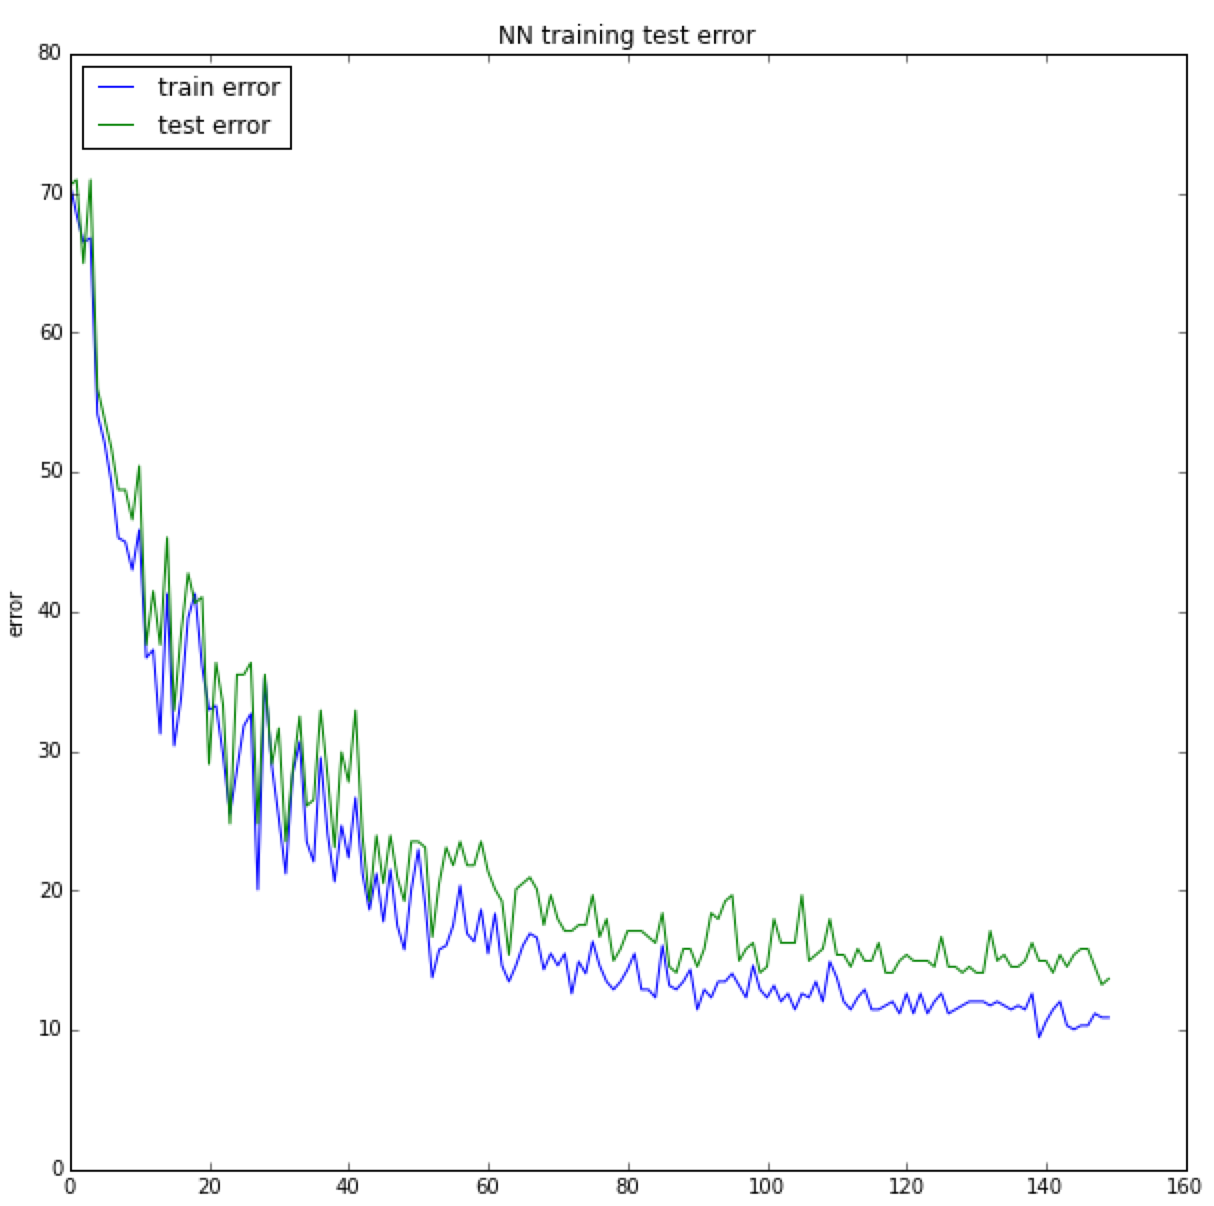
\includegraphics[width=0.6\linewidth]{img/graph003.png}
  \caption{Erreur d'entrainement et de test avec \texttt{training\_rate=0.003}}
  \label{graph003}
\end{figure}


En final la matrice de confusion est la suivantes:
\begin{figure}[h]
  \centering
    \includegraphics[width=0.6\linewidth]{img/mconf003.png}
  \caption{MAtrice de confusion final}
  \label{mconf003}
\end{figure}



